% Figure snippets — embed inline in main.tex

\begin{figure}[htbp]
\centering
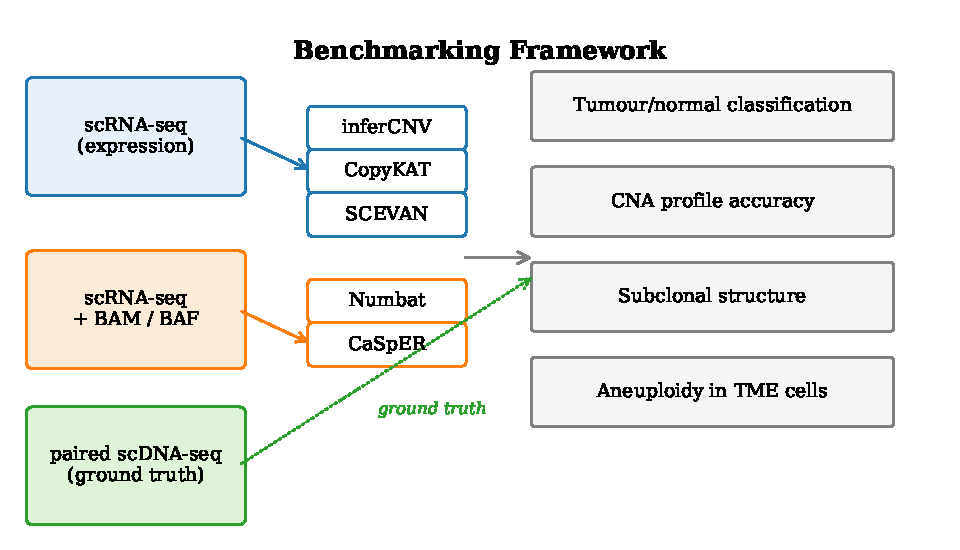
\includegraphics[width=0.9\textwidth]{figures/fig_workflow.pdf}
\caption{Overview of the benchmarking framework. Five scRNA-seq-based CNA
inference tools are evaluated in two methodological categories: expression-only
(inferCNV, CopyKAT, SCEVAN) and expression-plus-allele (Numbat, CaSpER).
Paired scDNA-seq from single-cell multi-omics datasets serves as ground truth
across four evaluation tasks: tumour/normal classification, CNA profile
accuracy, subclonal structure inference, and aneuploidy detection in
non-malignant cells.}
\label{fig:workflow}
\end{figure}

\begin{figure}[htbp]
\centering
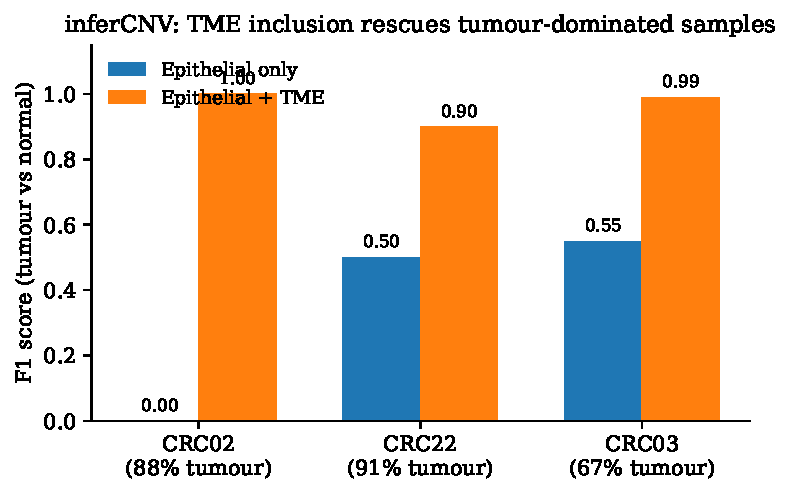
\includegraphics[width=0.7\textwidth]{figures/fig_tme_rescue.pdf}
\caption{Including tumour microenvironment (TME) cells rescues inferCNV F1
scores for tumour-normal classification in three CRC samples with high tumour
purity. For CRC02 (88\% tumour), CRC22 (91\%), and CRC03 (67\%), epithelial-only
F1 scores of 0, 0.5, and 0.55 rose to 1.0, 0.9, and 0.99 respectively when TME
cells were added to the input.}
\label{fig:tme_rescue}
\end{figure}

\begin{figure}[htbp]
\centering
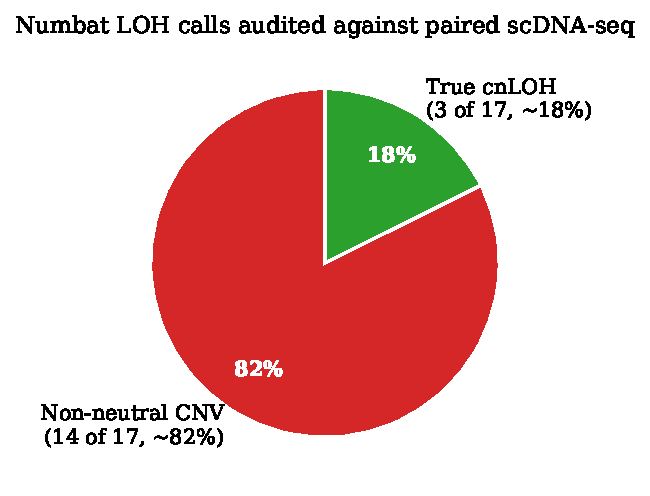
\includegraphics[width=0.55\textwidth]{figures/fig_loh_breakdown.pdf}
\caption{Audit of Numbat LOH calls against paired scDNA-seq allele-specific
copy number states. Of 17 LOH events reported by Numbat across multiple
samples, 14 ($\sim$82\%) were in fact non-neutral CNV events (amplifications
or deletions), while 3 corresponded to genuine copy-number-neutral LOH
(cnLOH).}
\label{fig:loh_breakdown}
\end{figure}

\begin{figure}[htbp]
\centering
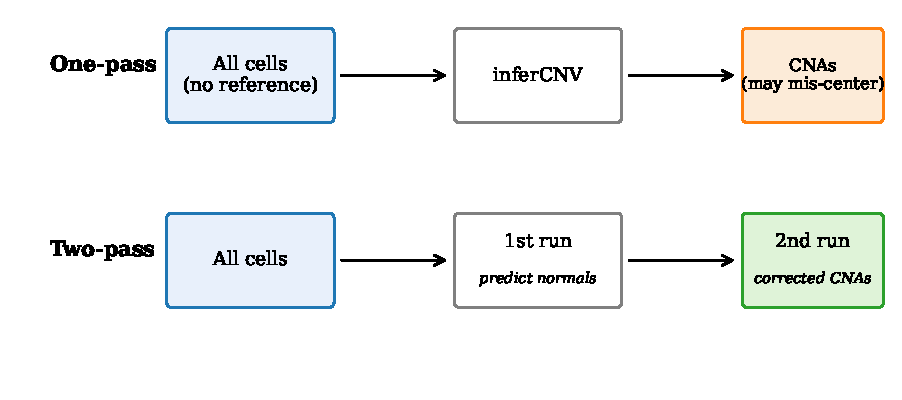
\includegraphics[width=0.9\textwidth]{figures/fig_two_pass.pdf}
\caption{One-pass versus two-pass inferCNV reference setting. In one-pass mode
(top) the whole cell population serves as its own reference, which can
mis-center copy number profiles when tumour purity is high. In two-pass mode
(bottom) cells predicted as normal in the first run are used as the reference
for a second run, yielding corrected CNA profiles.}
\label{fig:two_pass}
\end{figure}
